\chapter{Edit Filters as part of Wikipedia's socio-technical infrastructure}
\label{chap:filters}

%\section{Genesis}

``Abuse Filter is enabled'' reads the title of one of the eight stories of the March 23rd 2009 issue of English Wikipedia's newspaper, The Signpost~\cite{Signpost2009}.
``The extension allows all edits to be checked against automatic filters and heuristics, which can be set up to look for patterns of vandalism including page move vandalism and juvenile-type vandalism, as well as common newbie mistakes,'' the article proclaims.
%TODO something more from the signpost?

The extension, or at least its end user facing parts, was later renamed to ``edit filter'' in order to not characterise false positives as ``abuse'' and thus alienate good faith editors striving to improve the encyclopedia~\cite{Wikipedia:EditFilter},~\cite{Wikipedia:EditFilterTalkArchiveNameChange}.

In the present chapter, we aim to understand how edit filters work, who implements and runs them and above all, how and why they were introduced in the first place and what the qualitative difference is between them and other algorithmic quality control mechanisms.
%smth else we want to understand here?
%TODO come back at the end of the chapter and make sure, we answered these questions

\section{Data}

The foundations for the present chapter lie in EN Wikipedia's policies and guidelines.
Following pages were analysed in depth: \\
\url{https://en.wikipedia.org/wiki/Wikipedia:Edit_filter} \\
\url{https://en.wikipedia.org/wiki/Wikipedia_talk:Edit_filter/Archive_1} \\
<insert pages here>

%************************************************************************

\section{Definition}

According to EN Wikipedia's own definition, an edit filter is ``a tool that allows editors in the edit filter manager group to set controls mainly to address common patterns of harmful editing''~\cite{Wikipedia:EditFilter}.

A couple of keywords arouse interest here: %TODO make sure the chapter answered these questions
Who is in the edit filter manager group and how did they become part of it?
What controls exactly can be set?
What does ``mainly'' mean, are there other patterns addressed?
And what are the patterns of harmful editing addressed by the filters?

At least the ``mainly'' question is swiftly answered by the paragraph itself, since there is a footnote stating that ``[e]dit filters can and have been used to track or tag certain non-harmful edits, for example addition of WikiLove''~\cite{Wikipedia:EditFilter}.
We discuss (who is in) the edit filter manager group in section~\ref{section:who-can-edit} and the patterns of harmful editing (as well as some further non-harmful edit patterns) are inspected in detail in the next chapter.
Regarding the controls that can be set, we can briefly state that:
Every filter defines a regular expression (regex) pattern against which every edit made to Wikipedia is checked.
If there is a match, the edit in question is logged and potentially, additional actions such as tagging the edit summary, issuing a warning or disallowing the edit are invoked.
Both the regex patterns and the possible edit filter actions are investigated in greater detail in the following sections.

\subsection{Example of a filter}

For illustration purposes/better understanding, let us have a closer look at what a single edit filter looks like.
Edit filter with ID 365 is public and currently enabled (as of June 30th 2019).
This means the filter is working and everyone interested can view the filter's details.
Its description reads ``Unusual changes to featured or good content''.
The regex filter pattern is:
\begin{verbatim}
"page_namespace == 0 &
!(""confirmed"" in user_groups) &
old_size > 20000 & (
    ""#redirect"" in lcase(added_lines) |
    edit_delta < -15000 |
    edit_delta > 15000
) &
old_wikitext rlike
""\{\{([Ff]eatured|[Gg]ood)\s?article\}\}"""
\end{verbatim}
And the currently configured filter actions are: ``disallow''.

So, if a user whose status is not confirmed yet tries to edit a page in the article namespace which contains ``Featured'' or ``Good article'' and they either insert a redirect, delete 3/4 of the content or add 3/4 on top, the edit is automatically disallowed.

Note that an edit filter editor can easily change the action of the filter. (Or the pattern, as a matter of fact.)
The filter was last modified on October 23rd 2018.
All these details can be viewed on the filter's detailed page\footnote{\url{https://en.wikipedia.org/wiki/Special:AbuseFilter/365}}
or on the screenshot thereof (figure~\ref{fig:filter-details}) that I created for convenience.

Further information the filter detailed page displays is:
number of filter hits;
some statistics (the average time the filter takes to check an edit, percentage of hits and how many conditions from the condition limit it consumes);%TODO what is the condition limit
comments (left by filter editors, generally to log and explain changes);
flags (``Hide details of this filter from public view'', ``Enable this filter'', ``Mark as deleted'');
links to last modified (with diff and user who modified it), the edit filter's history and a tool for exporting the filter to another wiki;
and actions to take when the filter is triggered.

\begin{figure}
\centering
  \includegraphics[width=.9\paperwidth,height=.9\paperheight,keepaspectratio]{pics/detailed-page-filter365-no-boarder.png}
  \caption{Detailed page of edit filter \#365}~\label{fig:filter-details}
\end{figure}
%TODO graphic still looks weird..

%************************************************************************

\section{The AbuseFilter\footnote{Note that the user facing elements of this extention were renamed to ``edit filter'', however the extension itself, as well as its corresponding permissions, database tables etc. still reflect the original name.} Mediawiki extension}
\label{sec:mediawiki-ext}

At the end, from a technical perspective, Wikipedia's edit filters are a MediaWiki plugin that allows every edit (and some other editor's actions) to be checked against a speficied regular expression pattern before it is published.

The extension introduces following database tables where all data generated by it is stored: \emph{abuse\_filter}, \emph{abuse\_filter\_log}, \emph{abuse\_filter\_action} and \emph{abuse\_filter\_history}~\cite{gerrit-abusefilter-tables}.
\emph{abuse\_filter} contains detailed information about every filter.
\emph{abuse\_filter\_action} ... %TODO: Find out what this table is for!
Every update of a filter action, pattern, comments or other flags (whether the filter is enabled, hidden, deleted), etc. is recorded in \emph{abuse\_filter\_history}.
And every time a filter is triggered, the action that triggered it as well as further data such as the user who triggered the filter, their IP address, and a diff of the edit (if it was an edit), a timestamp, the title of the page the user was looking at, etc. are logged in \emph{abuse\_filter\_log}.

Most frequently, edit filters are triggered upon new edits, there are however further editor's actions that can trip an edit filter.
As of June 30th 2019, these include: \emph{edit}, \emph{move}, \emph{delete}, \emph{createaccount}, \emph{autocreateaccount}, \emph{upload}, \emph{stashupload}\footnote{See line 181 in \url{https://gerrit.wikimedia.org/r/plugins/gitiles/mediawiki/extensions/AbuseFilter/+/refs/heads/master/includes/special/SpecialAbuseLog.php}}.
%TODO explain what the actions are, especially the less obvious ones such as `autocreateaccount'
Historically, further editor's actions such as \emph{feedback}, \emph{gatheredit} and \emph{moodbar} could trigger an edit filter.
These are in the meantime deprecated. %TODO explain why? I have the guess that these are not available in the software anymore (generally, not only for the edit filters)

When a filter is triggered, beside logging the event in the \emph{abuse\_filter\_log} table (the only filter action which cannot be switched off), a further filter action may be invoked as well.
The plugin defines following possible filter actions:
\emph{tag}, \emph{throttle}, \emph{warn}, \emph{blockautopromote}, \emph{block}, \emph{degroup}, \emph{rangeblock}, \emph{disallow}\footnote{See line 2808 in \url{https://gerrit.wikimedia.org/r/plugins/gitiles/mediawiki/extensions/AbuseFilter/+/refs/heads/master/includes/AbuseFilter.php}}.
%TODO verify that none of the actions are deprecated; I have my doubts that for instance `revoking auto-promoted groups' may not be available anymore
The documentation of the AbuseFilter extension provides us comprehensive definitions for these~\cite{Mediawiki:AbuseFilterActions}:
\begin{itemize}
    \item \emph{tag}: The contribution is tagged with a specific tag (which can be defined and styled by the edit filter manager) which then appears on Recent Changes, contributions, logs, history pages, etc. and allows aggregations of lists for dashboards and similar.
    \item \emph{throttle}: The filter is activated upon the tripping of a rate limit. Configurable parameters are the allowed number of actions, the period of time in which these actions must occur, and how those actions are grouped. Actions can be grouped by user, IP address, /16 IP range, creation date of the user account, page, site, the edit count of the user or a combination thereof. (So trottling is something like ``do this if page X is edited more than Y times in Z seconds''.) %TODO do we need the explanation? is somewhat informal; also: does throttle do something on its own? or does it need an additional action?
     \item \emph{warn}: A warning is displayed that the edit may not be appreciated. (The warning message is configurable by the edit filter manager.) The editor who tripped the filter is provided with the opportunity to revise their edit and re-submit it. A link to the false positives page~\cite{Wikipedia:EditFilterFalsePositives} is also provided.
    \item \emph{blockautopromote}: The user who triggered the filter is banned from receiving extra groups from \$wgAutopromote for a random period of 3 to 7 days.
    \item \emph{block}: The user who triggered the filter is blocked indefinitely. An error message is displayed to inform the user of this action.
    \item \emph{degroup}: The user who triggered the filter is removed from all privileged groups (sysop, bureaucrat, etc). An error message is displayed to inform them of this action.
    \item \emph{rangeblock}: The entire /16 IP range from which the filter was triggered is blocked for a week.
    \item \emph{disallow}: An error message is shown to the editor informing them their edit was considered unconstructive and will not be saved. They are provided the opportunity to report a false positive.
\end{itemize}

\emph{rangeblock}, \emph{block}, \emph{degroup} and \emph{blockautopromote} haven't been used on the EN Wikipedia in recent years. %TODO: why? look for talk page archives around the last time they were used. Maybe there was a particular incident; nothing concerning autopromote in the EdiFilter talk page around 2012
% Isn't it rather that rangeblock, degroup and block have never been used on EN Wikipedia, at least according to the logs?
To be more precise, the last time filter actions other than \emph{log}, \emph{tag}, \emph{warn} or \emph{disallow} were triggered on the EN Wikipedia was in 2012 and these were \emph{blockautopromote} and \emph{aftv5flagabuse}. %TODO Refer to data analysis or make a quarry to back this
% Following 4 filters have blockautopromote as an action (note that this could have changed since 2012!): 115, 267, 334, 21;
\emph{aftv5flagabuse} is a deprecated action related to the now deprecated Article Feedback MediaWiki extension (or Article Feedback Tool, Version 5) which purpose was to involve readers more actively in article quality assessment\footnote{\url{https://www.mediawiki.org/w/index.php?title=Extension:ArticleFeedbackv5&oldid=3136840}}.
(However, during the testing phase, reader feedback was found mostly not particularly helpful and hence the extension was discontinued.)

Guidelines specifically call for careful use of \emph{disallow}.
Only severe cases for which ``substantially all good-faith editors would agree are undesirable'' or specific cases for which consensus has been reached should be disallowed~\cite{Wikipedia:EditFilter}.

Following new user permissions are introduced by the AbuseFilter plugin: %TODO quote \url{https://www.mediawiki.org/wiki/Extension:AbuseFilter} in a sensible manner, once it's decided on refs vs inline urls
\begin{itemize}
    \item \emph{abusefilter-modify}: ``Modify abuse filters''
    \item \emph{abusefilter-view}: ``View abuse filters''
    \item \emph{abusefilter-log}: ``View the abuse log''
    \item \emph{abusefilter-log-detail}: ``View detailed abuse log entries''
    \item \emph{abusefilter-private}: ``View private data in the abuse log''
    \item \emph{abusefilter-modify-restricted}: ``Modify abuse filters with restricted actions''
    \item \emph{abusefilter-modify-global}: ``Create or modify global abuse filters''
    \item \emph{abusefilter-revert}: ``Revert all changes by a given abuse filter''
    \item \emph{abusefilter-view-private}: ``View abuse filters marked as private''
    \item \emph{abusefilter-log-private}: ``View log entries of abuse filters marked as private''
    \item \emph{abusefilter-hide-log}: ``Hide entries in the abuse log''
    \item \emph{abusefilter-hidden-log}: ``View hidden abuse log entries''
    \item \emph{abusefilter-private-log}: ``View the AbuseFilter private details access log''
\end{itemize}

For additional reference, the format for the regex rules~\cite{Mediawiki:AbuseFilterRules}, the general documentation of the extension~\cite{Mediawiki:AbuseFilterExtension} as well as its source code~\cite{gerrit-abusefilter-source} can be consulted.


%************************************************************************

\section{History}
%TODO make sure there is enough explanation in the sections before to be able to follow the narrative here

Now that there is a general understanding of what edit filters look like today, let us take a step back and investigate how they came to be this way.
In order to comprehend the consensus building on the functionality of the extension, I sifted through the archives of the Edit Filter talk page\footnote{\url{https://en.wikipedia.org/w/index.php?title=Wikipedia_talk:Edit_filter/Archive_1&oldid=884572675}}
for the period between the announcement that the extension is planned up until the voting process preceding its introduction.

For a while at the beginnings of the discussion, there was some confusion among editors regarding the intended functionality of the edit filters.
Participants invoked various motivations for the introduction of the extension (which sometimes contradicted each other) and argued for or against the filters depending on these.
The discussion reflects a mix of ideological and practical concerns.
The biggest controversies lay along the lines of filters being public-vs-private and the actions the filters were to invoke upon a match.
An automated rights revokation or a block of the offending editor with no manual confirmation by a real person were of particular concern to a lot of editors (they were worried that the filters would not be able to understand context thus resulting in too many false positives and blocking many legitimate edits and editors).
As far as I understood, these features were technically implemented but never really used on English Wikipiedia (although there are \emph{blockautopromote} actions triggered in the \emph{abuse\_filter\_log}). %TODO investigate what exactly this means and why it hasn't happened since 2012

As to the public-vs-private debate, the initial plan was that all filters are hidden from public view and only editors with special permissions (the edit filter managers) were supposed to be able to view and modify the patterns and consult the logs.
The core developer of the extension was reasoning that its primary purpose was to fend off really persistent vandals with reasonable technical understanding who were ready to invest time and effort to circumvent anti-vandal measures
and that it was therefore unwise to make circumvention easier to them by allowing them to view the pattern according to which their edits were supressed.
This was however met with serious resistence by the community who felt that such secret extension was contradicting Wikipedia's values of openness and transparency.
Besides, opponents of the filters being completely private were concerned that the tool was quite powerful and hiding everything (syn!) will prevent the community from monitoring for errors and abuse.

Related to the above discussion, there was also disagreement regarding who was to have access to the newly developed tool.
Some felt access had to be granted more broadly in order for the tool to be effectively used.
They were reasoning that at least all administrators should be able to use it, since they already had the trust of the community.
Others feared that the admin group was quite broad already and access should be granted as carefully as possible since the extension had the potential to cause quite a lot of damage if used maliciously and it was ``not beyond some of our more dedicated trolls to "work accounts up" to admins, and then use them for their own purpose''.
This narrower option is how the right ended up to be governed.
%TODO where to put this? maybe a footnote?
(Although motivated trolls can potentially work up an account to any user rights, just my 2 cents.)

Another debated point was what the difference to bots (with admin rights) was and whether the extension was needed at all.
Apparently, there was some discontent with bot governance mirrored in the arguments for introducing the extension.
It was underlined that in contrast to admin bots the extension's source code was to be publicly available and well tested with more people (i.e. the edit filter managers) using and monitoring its functionality than the (usually) single bot operator responsible for a bot who, apparently, was oftentimes not responding to community concerns and emergencies fast enough (or at all).
On the other hand, there were yet again arguments, that the extension was supposed to indeed target the really malicious vandals not deterred by anti-vandalism measures already in force by preferably blocking them on the spot.

Others were asking what additional advantages the extension offered compared to semi-protection of pages which requires users to be autoconfirmed in order to be able to edit (normally meaning they have to have been registered for at least 4 days and have made at least 10 edits, but the restrictions are adjustable).
Here, User:Werdna was reasoning that the Edit Filters allow for fine-tuning of such restrictions and targeting offending editors in particular without making constraints unnecessarily strict for all users.

Although there were some diverging opinions on what the extension was supposed to target, in a nutshell, the motivation for its introduction seems to have been as follows:
Bots weren't reverting some kinds of vandalism fast enough, or, respectively, these vandalism edits required a human intervention and took more than a single click to get reverted.
These were mostly obvious but pervasive cases of vandalism, possibly introduced in a (semi-)automated fashion, that took some time and effort to clean up.
The motivation of the extention's developers was that if a filter just disallows such vandalism, vandal fighters could use their time more productively and check less obvious cases where more background knowledge/context is needed in order to decide whether an edit is vandalism or not.
According to the discussion archives, following types of edits were supposed to be targeted by the extension:\\
\url{https://en.wikipedia.org/wiki/Special:Contributions/Omm_nom_nom_nom}\\
%redirects to nonsensical names
\url{https://en.wikipedia.org/wiki/Special:Contributions/AV-THE-3RD}\\
\url{https://en.wikipedia.org/wiki/Special:Contributions/Fuzzmetlacker}\\


%************************************************************************

\section{Building a filter: the internal perspective}
\subsection{How is a new filter introduced?}

Only edit filter managers have the permissions necessary to implement filters, but anybody can propose new ones.
Every editor who notices some problematic behaviour they deem needs a filter can raise the issue at \url{https://en.wikipedia.org/wiki/Wikipedia:Edit_filter/Requested}.
The request can then be approved and implemented by an edit filter manager (mostly after a discussion/clarification of the details).
The Edit Filters Requests page asks users to go through the following checklist before requesting a filter:
\begin{itemize}
    \item problems with a single page are not suitable for an edit filter, since filters are applied to all edits;
    \item filters, after adding up, make editing slower, so the usefulness of every single filter and condition has to be carefully considered;
    \item in depth checks should be done by a separate software that users run on their own machines;
    \item no trivial errors should be catched by filters (e.g. concerning style guidelines);
    \item there are the Titles Blacklist\footnote{\url{https://en.wikipedia.org/w/index.php?title=MediaWiki:Titleblacklist&oldid=904314604}} and the Link/Spam Blacklist\footnote{\url{https://en.wikipedia.org/w/index.php?title=MediaWiki:Spam-blacklist&oldid=904319854}} which should be used if the issue at hand has to do with a problematic title or link.
\end{itemize}

For edit filter managers, the best practice way for introducing a new filter is described under \url{https://en.wikipedia.org/wiki/Wikipedia:Edit_filter/Instructions}.
According to the page, these steps should be followed:
\begin{enumerate}
    \item read the documentation: \url{https://www.mediawiki.org/wiki/Extension:AbuseFilter/Rules_format}
    \item test with debugging tools: \url{https://en.wikipedia.org/wiki/Special:AbuseFilter/tools} (visible only for users who are already in the edit filter managers user group)
    \item test with the batch testing interface (also available to edit filter managers only)
    \item create a logging only filter: \url{https://en.wikipedia.org/wiki/Special:AbuseFilter/new} (edit filter manager permissions needed)
    \item announce the filter at the edit filter notice board~\cite{Wikipedia:EditFilterNoticeboard}, so other edit filter managers can comment on it
    \item finally, fully enable the filter by adding an appropriate additional edit filter action.
\end{enumerate}

Performance seems to be fairly important for the edit filter system:
On multiple occasions, there are notes on recommended order of operations, so that the filter evaluates as resource sparing as possible~\cite{Wikipedia:EditFilterInstructions} or invitations to consider whether an edit filter is the most suitable mechanism for solving a particular issue at all~\cite{Wikipedia:EditFilter},~\cite{Wikipedia:EditFilterRequested}.
%TODO maybe that's the best place to explain the condition limit?

According to the documentation, step 4 from the checklist can be skipped in ``urgent situations'' and corresponding filters can have more severe actions enabled directly. %TODO check whether comparative of "severe" is "more severe" or "severer"
In such case, the editor introducing the filter has to closely monitor the logs for potential filter misconduct.
However, the guidelines do not elaborate on what exactly constitutes a ``urgent situation''.
Unfortunately, investigating potential pitfalls of this provision is beyond the scope of the present work and one of the directions for further studies suggested in section~\ref{sec:further-studies}.

Edit filter managers often introduce filters based on some phenomena they have observed caught by other filters, other algorithmic quality control mechanisms or general experience.
As all newly implemented filters, these are initially enabled in logging only mode until enough log entries are generated to evaluate whether the incident is severe and frequent enough to need a filter.
%TODO this actually fits also in the patterns of new filters in chap.5; these are the filters introduced for couple of days/hours, then switched off to never be enabled again


\subsection{Who can edit filters?}
\label{section:who-can-edit}

In order to be able to set up an edit filter on their own, an editor needs to have the \emph{abusefilter-modify} permission (which makes them part of the edit filter manager group).
According to~\cite{Wikipedia:EditFilter} this right is given only to editors who ``have the required good judgment and technical proficiency''.
Further down on the page it is clarified that it is administrators who can assign the permission to users (also to themselves) and they should only assign it to non-admins in exceptional cases, ``to highly trusted users, when there is a clear and demonstrated need for it''.
If editors wish to be given this permission, they can hone and prove their skills by helping with requested edit filters and false positives~\cite{Wikipedia:EditFilter}.

The formal process for requesting the \emph{abusefilter-modify} permission is to raise the request at the edit filter noticeboard~\footnote{\url{https://en.wikipedia.org/w/index.php?title=Wikipedia:Edit_filter_noticeboard&oldid=904205276}}.
A discussion is held there, usually for 7 days, before a decision is reached~\cite{Wikipedia:EditFilter}.

As of 2017, when the ``edit filter helper'' group was introduced (editors in this group have the \emph{abusefilter-view-private} permission)\footnote{\url{https://en.wikipedia.org/w/index.php?title=Wikipedia:Edit_filter_helper&oldid=878127027}},
the usual process seems to be that editors request this right first and only later the full \emph{abusefilter-modify} permissions\footnote{That is the tendency we observe at \url{https://en.wikipedia.org/w/index.php?title=Wikipedia:Edit_filter_noticeboard&oldid=904205276 }}.

A list of the current edit filter managers for the EN Wikipedia can be found here: \url{https://en.wikipedia.org/wiki/Special:ListUsers/abusefilter}.
As of May 10, 2019, there are 154 users in the ``edit filter managers'' group\footnote{\url{https://en.wikipedia.org/w/index.php?title=Special:ListUsers&offset=&limit=250&username=&group=abusefilter&wpsubmit=&wpFormIdentifier=mw-listusers-form}}.
(For comparison, as of March 9, 2019 there are 1181 admins, see \url{https://en.wikipedia.org/w/index.php?title=Special:ListUsers/sysop}.)
Out of the 154 edit filter managers only 11 are not administrators (most of them have other privileged groups such as ``rollbacker'', ``pending changes reviewer'', ``extended confirmed user'' and similar though).

Some of the edit filter managers are also bot operators.
The interesting patterns of collaboration between the two technologies are discussed in section~\ref{subsection:collaboration-bots-filters}.

%************************************************************************

\section{Filters during runtime: the external perspective}

%TODO: Flowchart of the filtering process!

\subsection{What happens when an editor triggers an edit filter? Do they notice this at all?}

As described section~\ref{sec:mediawiki-ext}, a variety of different actions may occur when a filter gets tripped.
Of these, only \emph{tag}, \emph{throttle}, \emph{warn}, and \emph{disallow} seem to be used today.
If a filter is set to \emph{warn} or \emph{disallow}, the editor is notified that they hit a filter by a warning message (see figure~\ref{fig:screenshot-warn-disallow}).
These warnings describe the problem that occurred and present the editor with possible paths of action:
complain on the False Positives page\footnote{\url{https://en.wikipedia.org/w/index.php?title=Wikipedia:Edit_filter/False_positives&oldid=879367604}} in case of \emph{disallow} (the edit is not saved),
or, complain on the False Positives page and publish the change anyway in case of \emph{warn}.
(Of course, in case of a warning, the editor can modify their edit before publishing it.)
On the other hand, when the filter action is set to \emph{tag} or \emph{log} only, the editor doesn't really notice they tripped a filter unless they are looking more closely.
Tagged edits are marked as such in the page's revision history for example (see figure~\ref{fig:tags-in-history})
and all edits that trigger an edit filter are listed in the Abuse Log\footnote{\url{https://en.wikipedia.org/wiki/Special:AbuseLog}} (see figure~\ref{fig:screenshot-abuse-log}).
%TODO How about throttling: the AbuseLog is currently timing out when I try to filter entries according to action(=throttle)

\begin{figure}
\centering
  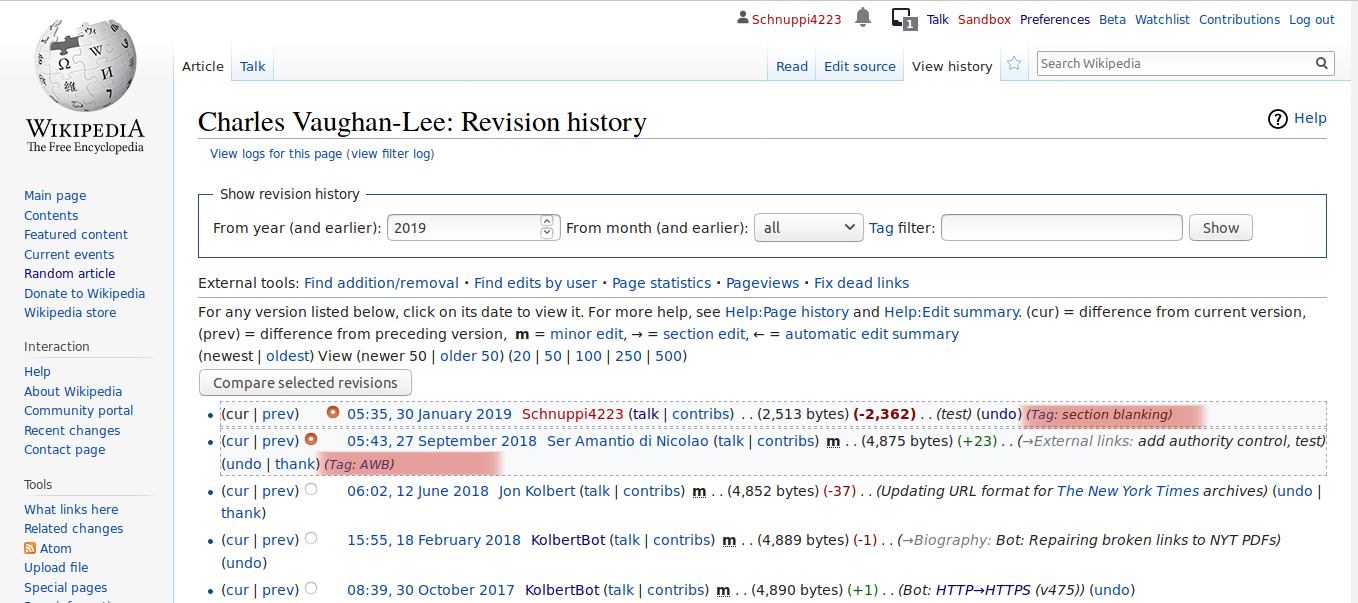
\includegraphics[width=0.9\columnwidth]{pics/screenshots-filter-trigger/Screenshot-tags-in-revision-history.png}
  \caption{Tagged edits are marked as such in a page's revision history}~\label{fig:tags-in-history}
\end{figure}

\begin{figure}
\centering
  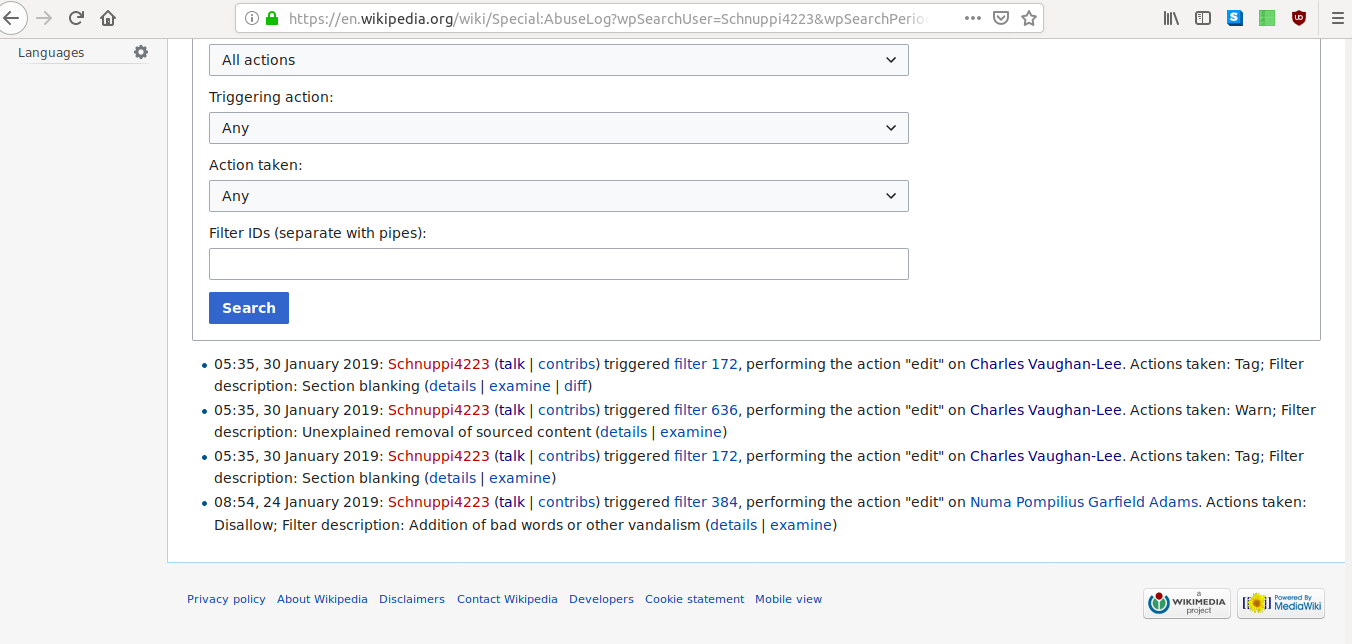
\includegraphics[width=0.9\columnwidth]{pics/screenshots-filter-trigger/Screenshot-abuse-log.png}
  \caption{Abuse Log showing all filter triggers by User:Schnuppi4223}~\label{fig:screenshot-abuse-log}
\end{figure}

\begin{figure}
\centering
  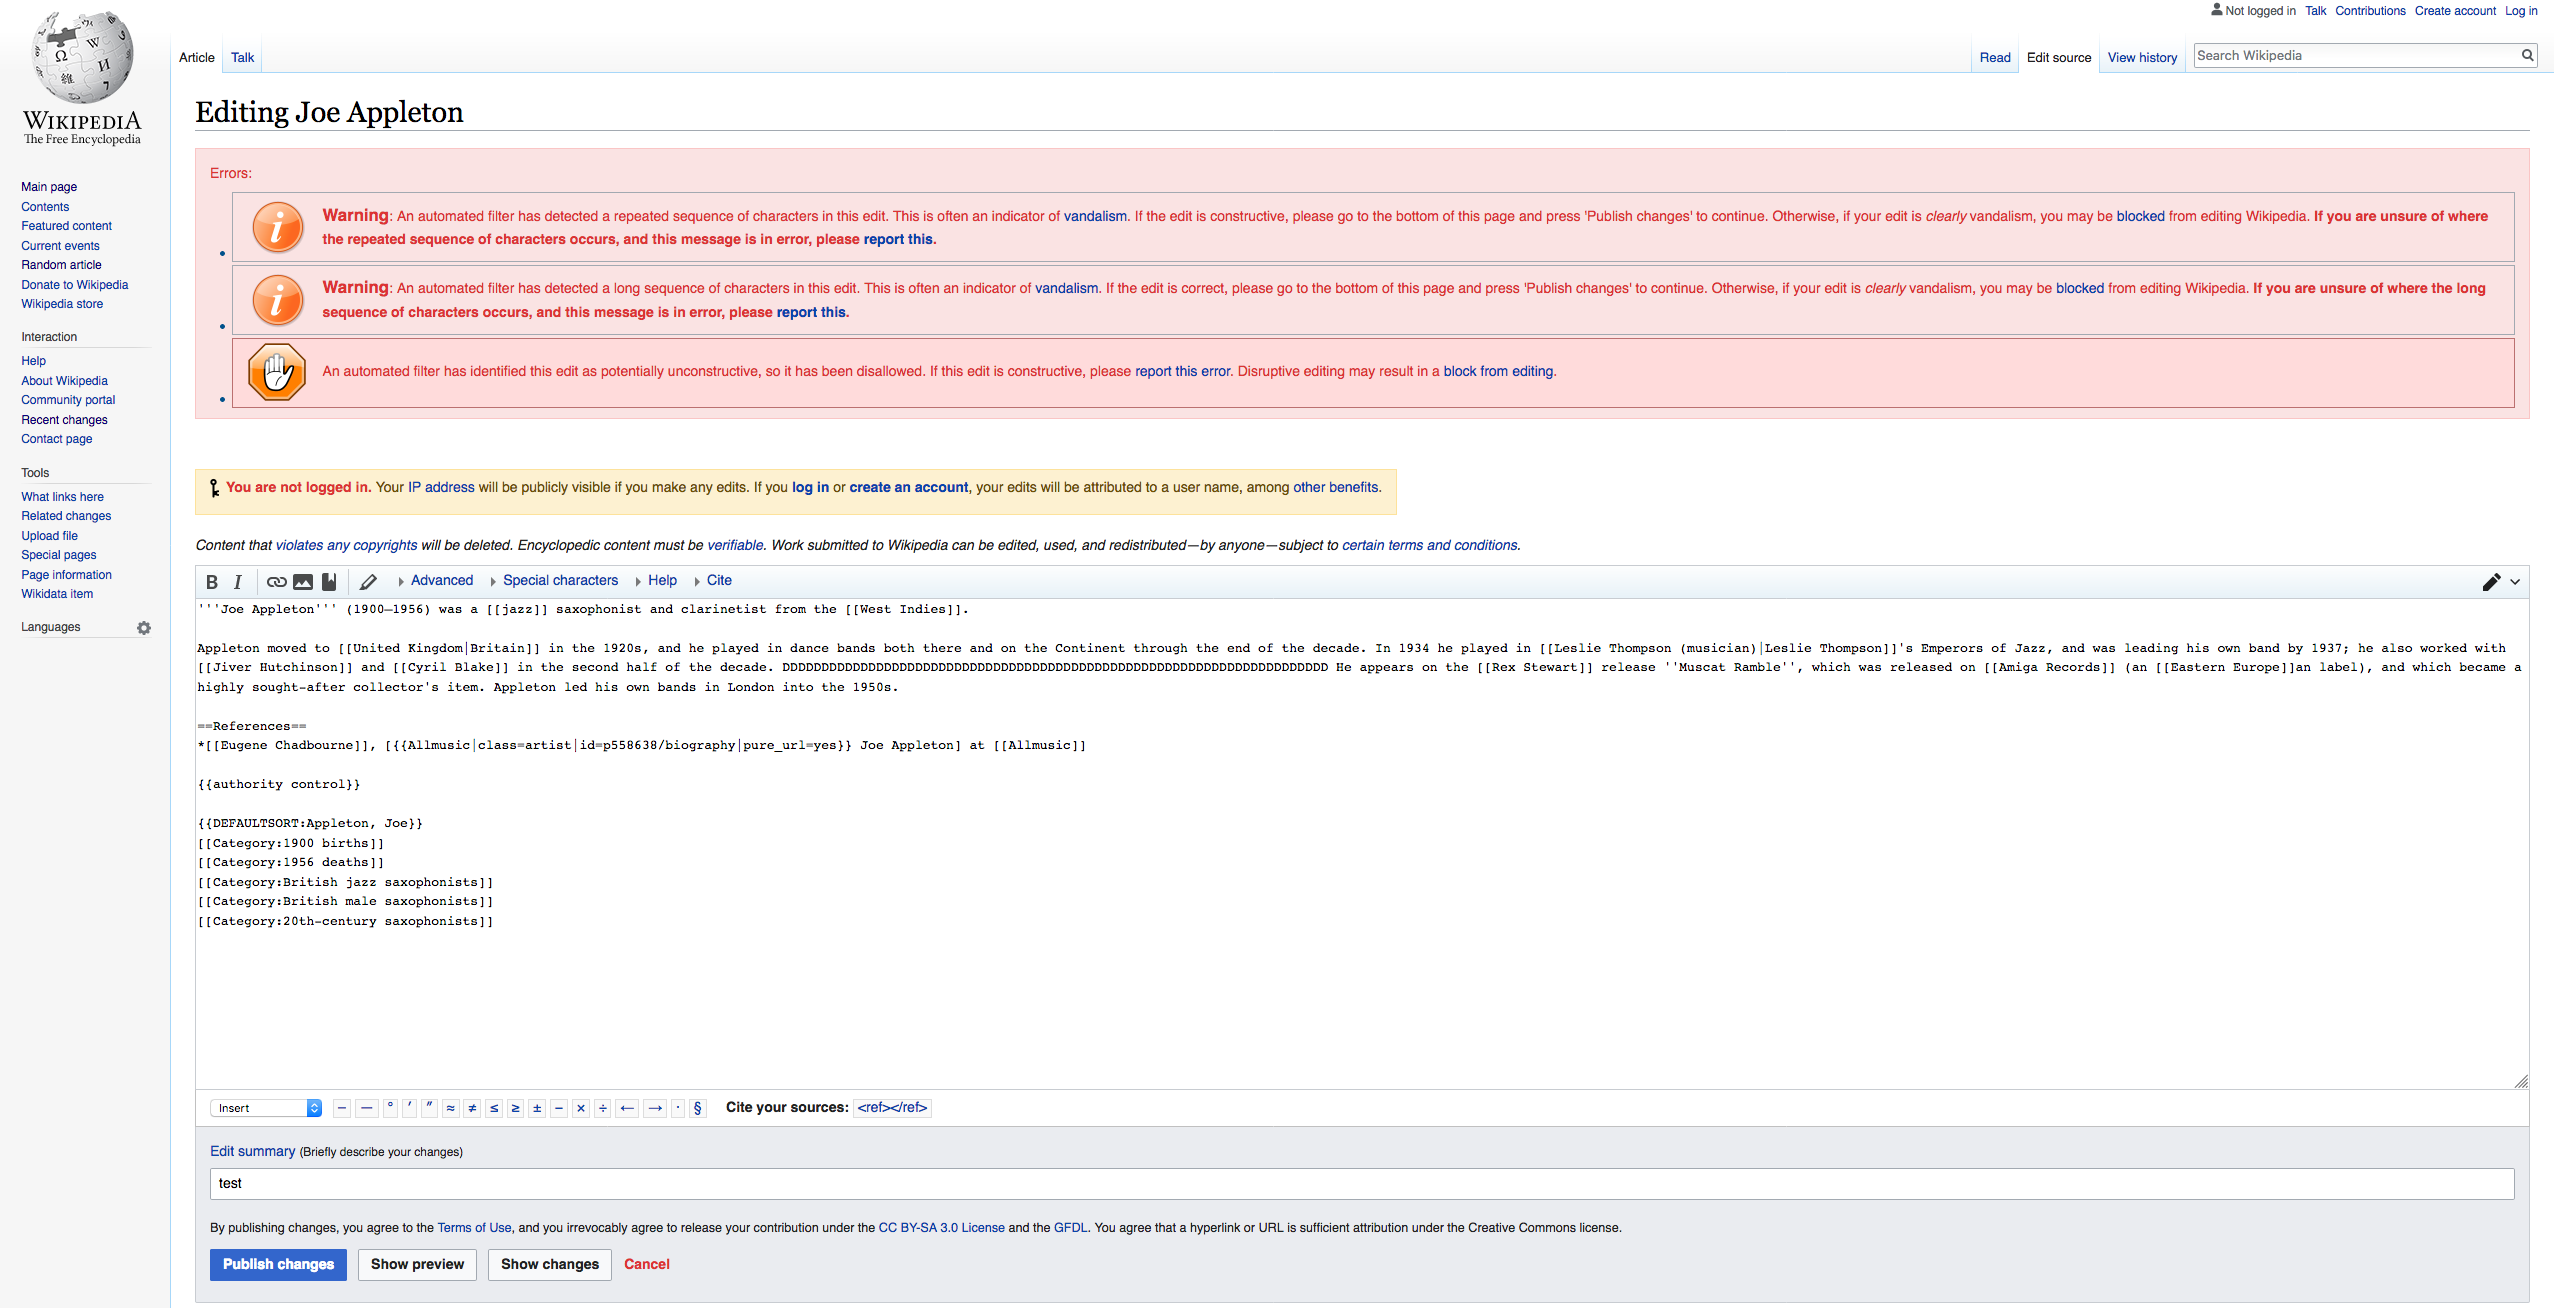
\includegraphics[width=0.9\columnwidth]{pics/screenshots-filter-trigger/Screenshot-trigger-warning-filter.png}
  \caption{Editor gets notified their edit triggered multiple edit filters}~\label{fig:screenshot-warn-disallow}
\end{figure}


\subsection{How are problems handled?}

There are several pages where problematic behaviour concerning edit filters are reported and potential solutions are considered.

For instance, current filters behaviour is discussed on the Edit Filter Noticeboard~\footnote{\url{https://en.wikipedia.org/w/index.php?title=Wikipedia:Edit_filter_noticeboard&oldid=904205276}}.
Issues handled here include changing the edit filter action of single filters, changing edit filter warning templates, problems with specific regexes or variables and proposals for filter deletions (or for introducing new filters).
Furthermore, on the noticeboard discussions take place about giving edit filter manager rights to users, or withdrawing these if a misuse was observed and raising the issue with the editor directly didn't resolve the problem~\cite{Wikipedia:EditFilter}.

False positives among the filter hits are reported and discussed on a separate page~\footnote{\url{https://en.wikipedia.org/w/index.php?title=Wikipedia:Edit_filter/False_positives&oldid=879367604}}.
Edit filter managers and other interested editors monitor this page and verify or disprove the reported incidents.
Edit filter managers use true false positives to improve the filters, give advice to good faith editors who tripped a filter and discourage authors of vandalism edits who reported these as false positives from continuing with their disrtuption.
% who moderates the false positives page? where does the info come from that it is edit filter managers? I think this info comes from observation

Moreover, edit filter managers are advised to consult and comply with personal security best practices (such as choosing a strong password and using two-factor authentication).
If their account is compromised, they lose their edit filter manager rights and get blocked, since this threatens site security.
Edit filter managers are encouraged to actively report problems with their account so that in case of doubt these can be blocked~\cite{Wikipedia:EditFilter}.

%************************************************************************

\section{Edit filters' role in the quality control frame}
%TODO do we need this chapter and extra fazit? I'm inclined to do fazit here

The purpose of the present section is to review what we have learnt so far and summarise/outline how edit filters fit in Wikipedia's quality control ecosystem.

\begin{comment}
    Recap questions relevant for this chapter:
* Why are there mechanisms triggered before an edit gets published (such as edit filters), and such triggered afterwards (such as bots)? Is there a qualitative difference?

Q1 We wanted to improve our understanding of the role of filters in existing algorithmic quality-control mechanisms (bots, ORES, humans).

From l.12
In the present chapter, we aim to understand how edit filters work, who implements and runs them and above all, how and why they were introduced in the first place and what the qualitative difference is between them and other algorithmic quality control mechanisms.
\end{comment}

As the timeline in figure~\ref{fig:timeline} shows, the time span in which algorithmic quality control mechanisms (first vandal fighting bots and semi-automated tools and later filters) were introduced fits logically the period after the exponential growth of Wikipedia took off.
The rapidly increasing workload could not be feasibly handled manually anymore and the community turned to technical solutions.
As shown elsewhere (cite Halfaker, someone else?), this turn (syn!) had a lot of repercussions:
one of the most severe of them being that newcomers' edits were reverted stricter than before (accepted or rejected on a yes-no basis with the help of automated tools, instead of manually seeking to improve the contributions and ``massage'' them into an acceptable form), which in consequence drove a lot of them away.

%TODO overlay with exponential growth diagram
\begin{table}
    \begin{tabular}{ r | p{.8\textwidth}}
   Oct 2001 & automatically import entries from Easton’s Bible Dictionary by a script \\
29 Mar 2002 & First version of \url{https://en.wikipedia.org/wiki/Wikipedia:Vandalism} (WP Vandalism is published) \\
   Oct 2002 & RamBot \\
       2006 & BAG was first formed \\
13 Mar 2006 & 1st version of Bots/Requests for approval is published: some basic requirements (also valid today) are recorded \\
28 Jul 2006 & VoABot II ("In the case were banned users continue to use sockpuppet accounts/IPs to add edits clearly rejected by consensus to the point were long term protection is required, VoABot may be programmed to watch those pages and revert those edits instead. Such edits are considered blacklisted. IP ranges can also be blacklisted. This is reserved only for special cases.") \\
21 Jan 2007 & Twinkle Page is first published (empty), filled with a basic description by beginings of Feb 2007 \\
24 Jul 2007 & Request for Approval of original ClueBot \\
16 Jan 2008 & Huggle Page is first published (empty) \\
18 Jan 2008 & Huggle Page is first filled with content \\
23 Jun 2008 & 1st version of Edit Filter page is published: User:Werdna announces they're currently developing the extention \\
 2 Oct 2008 & \url{https://en.wikipedia.org/wiki/Wikipedia_talk:Edit_filter} was first archived; its last topic was the voting for/against the extention which seemed to have ended end of Sep 2008 \\
   Jun 2010 & STiki initial release \\
20 Oct 2010 & ClueBot NG page is created \\
11 Jan 2015 & 1st commit to github ORES repository \\
30 Nov 2015 & ORES paper is published
    \end{tabular}
    \caption{Timeline: Introduction of algorithmic quality control mechanisms}~\label{fig:timeline}
\end{table}

% Comparison of the mechanisms: each of them has following salient characteristics

% Discussion of the table (fließtext)
\begin{comment}
From the Edit filter talk archives:
"Firstly, I must note that the code of the extension itself will be public in the MediaWiki subversion repository, that the filters will be editable by anyone with the appropriate privileges, and that it would be very simple to disable any user's use of the filtering system, any particular filter, or, indeed, the entire extension. This is quite different from, say, an anti-vandalism adminbot. The code is private, and, in any case, too ugly for anybody to know how to use it properly. The code can only be stopped in real terms if somebody blocks and desysops the bot, and the bot is controlled by a private individual, with no testing.

In this case, there are multiple hard-coded safeguards on the false positive rate of individual filters, and the extension itself will be well-tested. In addition, I suggest that a strong policy would be developed on what the filters can be used to do, and on what conditions they can match on: I've developed a little system which tests a filter on the last several thousand edits before allowing it to be applied globally."

    So, this claims that filters are open source and will be a collaborative effort, unlike bots, for which there is no formal requirement that the code is public (although in recent years, it kinda is, compare BAG and approval requirements).
    Also, the extension allows multiple users to work on the same filters and there are tests. Unlike bots, which are per definition operated by one user.

    "We're not targetting the 'idiots and bored kids' demographic, we're targetting the 'persistent vandal with a known modus operandi and a history of circumventing prevention methods' demographic. — Werdna • talk 07:28, 9 July 2008 (UTC)"

"It is designed to target repeated behaviour, which is unequivocally vandalism. For instance, making huge numbers of page moves right after your tenth edit. For instance, moving pages to titles with 'HAGGER?' in them. All of these things are currently blocked by sekrit adminbots. This extension promises to block these things in the software, allowing us zero latency in responding, and allowing us to apply special restrictions, such as revoking a users' autoconfirmed status for a period of time."

Also from the archives, ausformuliert, use towards describing the table:
Further advantages of the extension highlighted by its proponents/supporters were that it had no latency, reacting immediately when an offending edit is happening and thus not allowing abusive content to be public at all.
Besides, they were reasoning, it was to be part of the core software, so there was no need for renting extra server resources where an external script/bot can run, thus ensuring immediate response and less extra work.
The advantages over anti-vandal bots and other tools were seen to be ``speed and tidiness''.

\end{comment}
\begin{comment}
\url{http://www.aaronsw.com/weblog/whorunswikipedia}
"But what’s less well-known is that it’s also the site that anyone can run. The vandals aren’t stopped because someone is in charge of stopping them; it was simply something people started doing. And it’s not just vandalism: a “welcoming committee” says hi to every new user, a “cleanup taskforce” goes around doing factchecking. The site’s rules are made by rough consensus. Even the servers are largely run this way — a group of volunteer sysadmins hang out on IRC, keeping an eye on things. Until quite recently, the Foundation that supposedly runs Wikipedia had no actual employees.
This is so unusual, we don’t even have a word for it. It’s tempting to say “democracy”, but that’s woefully inadequate. Wikipedia doesn’t hold a vote and elect someone to be in charge of vandal-fighting. Indeed, “Wikipedia” doesn’t do anything at all. Someone simply sees that there are vandals to be fought and steps up to do the job."
//yeah, I'd call it "do-ocracy"

Reflections on the archive discussion
So, to summarise once again. Problem is blatant vandalism, which apparently doesn't get reverted fast enough.
Human editors are not very fast in general and how fast it is solving this with a bot depends on how often the bot runs and what's its underlying technical infrastructure (e.g. I run it on my machine in the basement which is probably less robust than a software extension that runs on the official Wikipedia servers).

\end{comment}

Following table summarises the aspects of Wikipedia's various algorithmic quality control mechanisms:
\begin{landscape}
    \begin{longtable}{ | p{3cm} | p{4.5cm} | p{4.5cm} | p{4.5cm} | p{4.5cm} | }
    \hline
               & Filters & Bots & Semi-Automated tools & ORES \\
    \hline
    \multirow{7}{*}{Properties} &  based on REGEXes & rule/ML based & rule/ML based & ML framework \\
                               &  part of the "software" (MediaWiki plugin)  &  run on user's infrastructure ("bespoke code") & extra infrastructure & not used directly, can be incorporated in other tools \\
                               & extension is open source & no requirement for code to be public & heuristics obfuscated by the interface & open source \\
                               & public filters directly visible for anyone interested & & & \\
                               & trigger \emph{before} an edit is published & trigger after an edit is published & trigger after an edit is published & \\
                               & zero latency, trigger immediately & latency varies & generally higher latency than bots & \\
                               & collaborative effort & mostly single dev/operator (recently: bot frameworks) & few devs & few devs \\
    \hline
    \multirow{2}{*}{People involved} & edit filter managers (EN Wiki) & no special rights needed (except for admin bots) & \emph{rollback} permission needed & mostly Scoring Platform team \\
                                     & & bot gets a ``bot flag'' & & \\
    \hline
        \multirow{2}{*}{Hurdles to participate} & gain community trust to become an edit filter manager & get approval from the BAG & get a \emph{rollback} permission& \\
                                            & understand REGEXes & programming knowledge, understand APIs, ... & get familiar with the tool & understand ML \\
    \hline
        \multirow{2}{*}{Concerns} & censorship infrastructure & ``botophobia'' & gamification & general ML concerns: hard to understand \\
                                  & powerful, can in theory block editors based on (hidden) filters & & & \\
    \hline
        Areas of application & & & & \\
    \hline
\end{longtable}
\end{landscape}
%TODO: explain table with text, give table caption

\begin{comment}
\begin{verbatim}
                     | Filters                          | Bots                          |  Semi-Automated tools   |  ORES
--------------------------------------------------------------------------------------------------------------------------------------------
                     |                                  |                               |                         |
                     | - based on REGEXes               | - rule/ML based               | - rule/ML based         | - ML framework
properties           | - part of the "software"/        | - "bespoke code": run on      | - heuristics obfusca-   | - not used directly, but can
                     |   platform (MediaWiki ext)       |   user's infrastructure       |   ted by the interface  |   instead be incorporated in
                     | - public filters are directly    | - no requirement for the code |   (but often configura- |   other tools
                     |   visible for everyone           |   to be made public           |   ble to an extent)     |
                     |   interested                     | - you can relatively easily   | - mostly based on a     |
                     | - trigger *before* an edit is    |   get all the filters; you    |   centralised queue     |
                     |   published                      |   cannot easily get all bots  | - trigger after an edit |
                     | - source code of the extension   | - trigger after an edit is    |   is published          |
                     |   is publicly viewable           |   published                   |                         |
                     | - zero latency, triggered imme-  | - latency varies              |                         |
                     |   diately                        |                               |                         |
                     | - collaborative effort           | - mostly single dev/operator  |                         |
                     |                                  |   (although in recent years a |                         |
                     |                                  |   lot of bots rely on bot     |                         |
                     |                                  |   frameworks)                 |                         |
                     |                                  |                               |                         |
---------------------|------------------------------------------------------------------------------------------------------------------------
                     |                                  |                               |                         |
                     | - edit filter managers           | - no special persmissions/    | - *rollback* perm       | - mostly Scoring platform
                     |  group (EN Wiki)                 |   rights needed               |                         |   team (?)
Who does this?       |  (abusefilter-modify perm)       | - a bot gets a bot flag       |                         |
                     |                                  |                               |                         |
---------------------|------------------------------------------------------------------------------------------------------------------------
                     |                                  |                               |                         |
                     | - become an edit filter manager  | - get an approval to run the  | - learn the tool        | - understand ML
What are the hurdles | - you have to *only* understand  |   bot from the BAG            | - install Windows^^     | - formal requirements to
to participate       |   REGEXes (relatively simple?    | - programming knowledge       |   (some don't support   |   develop ORES?
                     |   although relatively fast quite | - understand APIs, ..         |   other OS)             |
                     |   confusing)                     | - (but there is a lot to      | - get the rollback perm |
                     |                                  |   understand with all the     |                         |
                     |                                  |   mechanisms)                 |                         |
                     |                                  |                               |                         |
-----------------------------------------------------------------------------------------------------------------------------------------------
                     |                                  |                               |                         |
                     | - censorship infrastructure?     | - "botophobia"                | - gamification          | - general ML concerns:
Concerns             | - powerful, can in theory block  |                               |                         |   hard to understand
                     |   editors based on hidden        |                               |                         |
                     |   filters                        |                               |                         |
                     |                                  |                               |                         |
------------------------------------------------------------------------------------------------------------------------------------------------
                     |
Application areas    |
                     |
------------------------------------------------------------------------------------------------------------------------------------------------
\end{verbatim}
\end{comment}

% When is which mechanism used
\subsection{Alternatives to Edit Filters}
%TODO is this the most suitable place for this? If yes, write a better preamble

Since edit filters run against every edit saved on Wikipedia, it is generally adviced against rarely tripped filters and a number of alternatives is offered to edit filter managers and editors proposing new filters.
For example, there is the page protection mechanism that addresses problems on a single page.
suitable for handling a higher number of incidents concerning single page.
Also, title and spam blacklists exist and these might be the way to handle disruptive page titles or link spam~\cite{Wikipedia:EditFilter}.
Moreover, it is recommended to run in-depth checks (for single articles) separately, e.g. by using bots~\cite{Wikipedia:EditFilterRequested}.

%********************
% Filters vs bots
% Investigation of edit filter managers who are also bot operators: what do they implement when?
\begin{comment}
Question:
Oftentimes edit filter managers are also bot operators; how would they decide when to implement a filter and when a bot?
%TODO: ask people! (on IRC?)
I've compiled a list of edit filter managers who are simultaneously also bot operators;
I've further assembled the bots they run and made notes on the bots that seem to be relevant to vandalism prevention/quality assurance
I'm currently trying to determine from document traces what filter contributions the corresponding edit filter managers had and whether they are working on filters similar to the bots they operate.
Insight is currently minimal, since abuse\_filter\_history table is not available and we can only determine what filters an edit filter manager has worked on from limited traces such as: last modifier of the filter from abuse\_filter table; editors who signed their comments from abuse\_filter table; probably some noticeboards or talk page archives, but I haven't looked into these so far.
\end{comment}
%**********************
So, as shown in figure~\ref{fig:funnel-with-filters}, edit filters are crucial since they get active before any of the other mechanisms.

\begin{figure}
\centering
  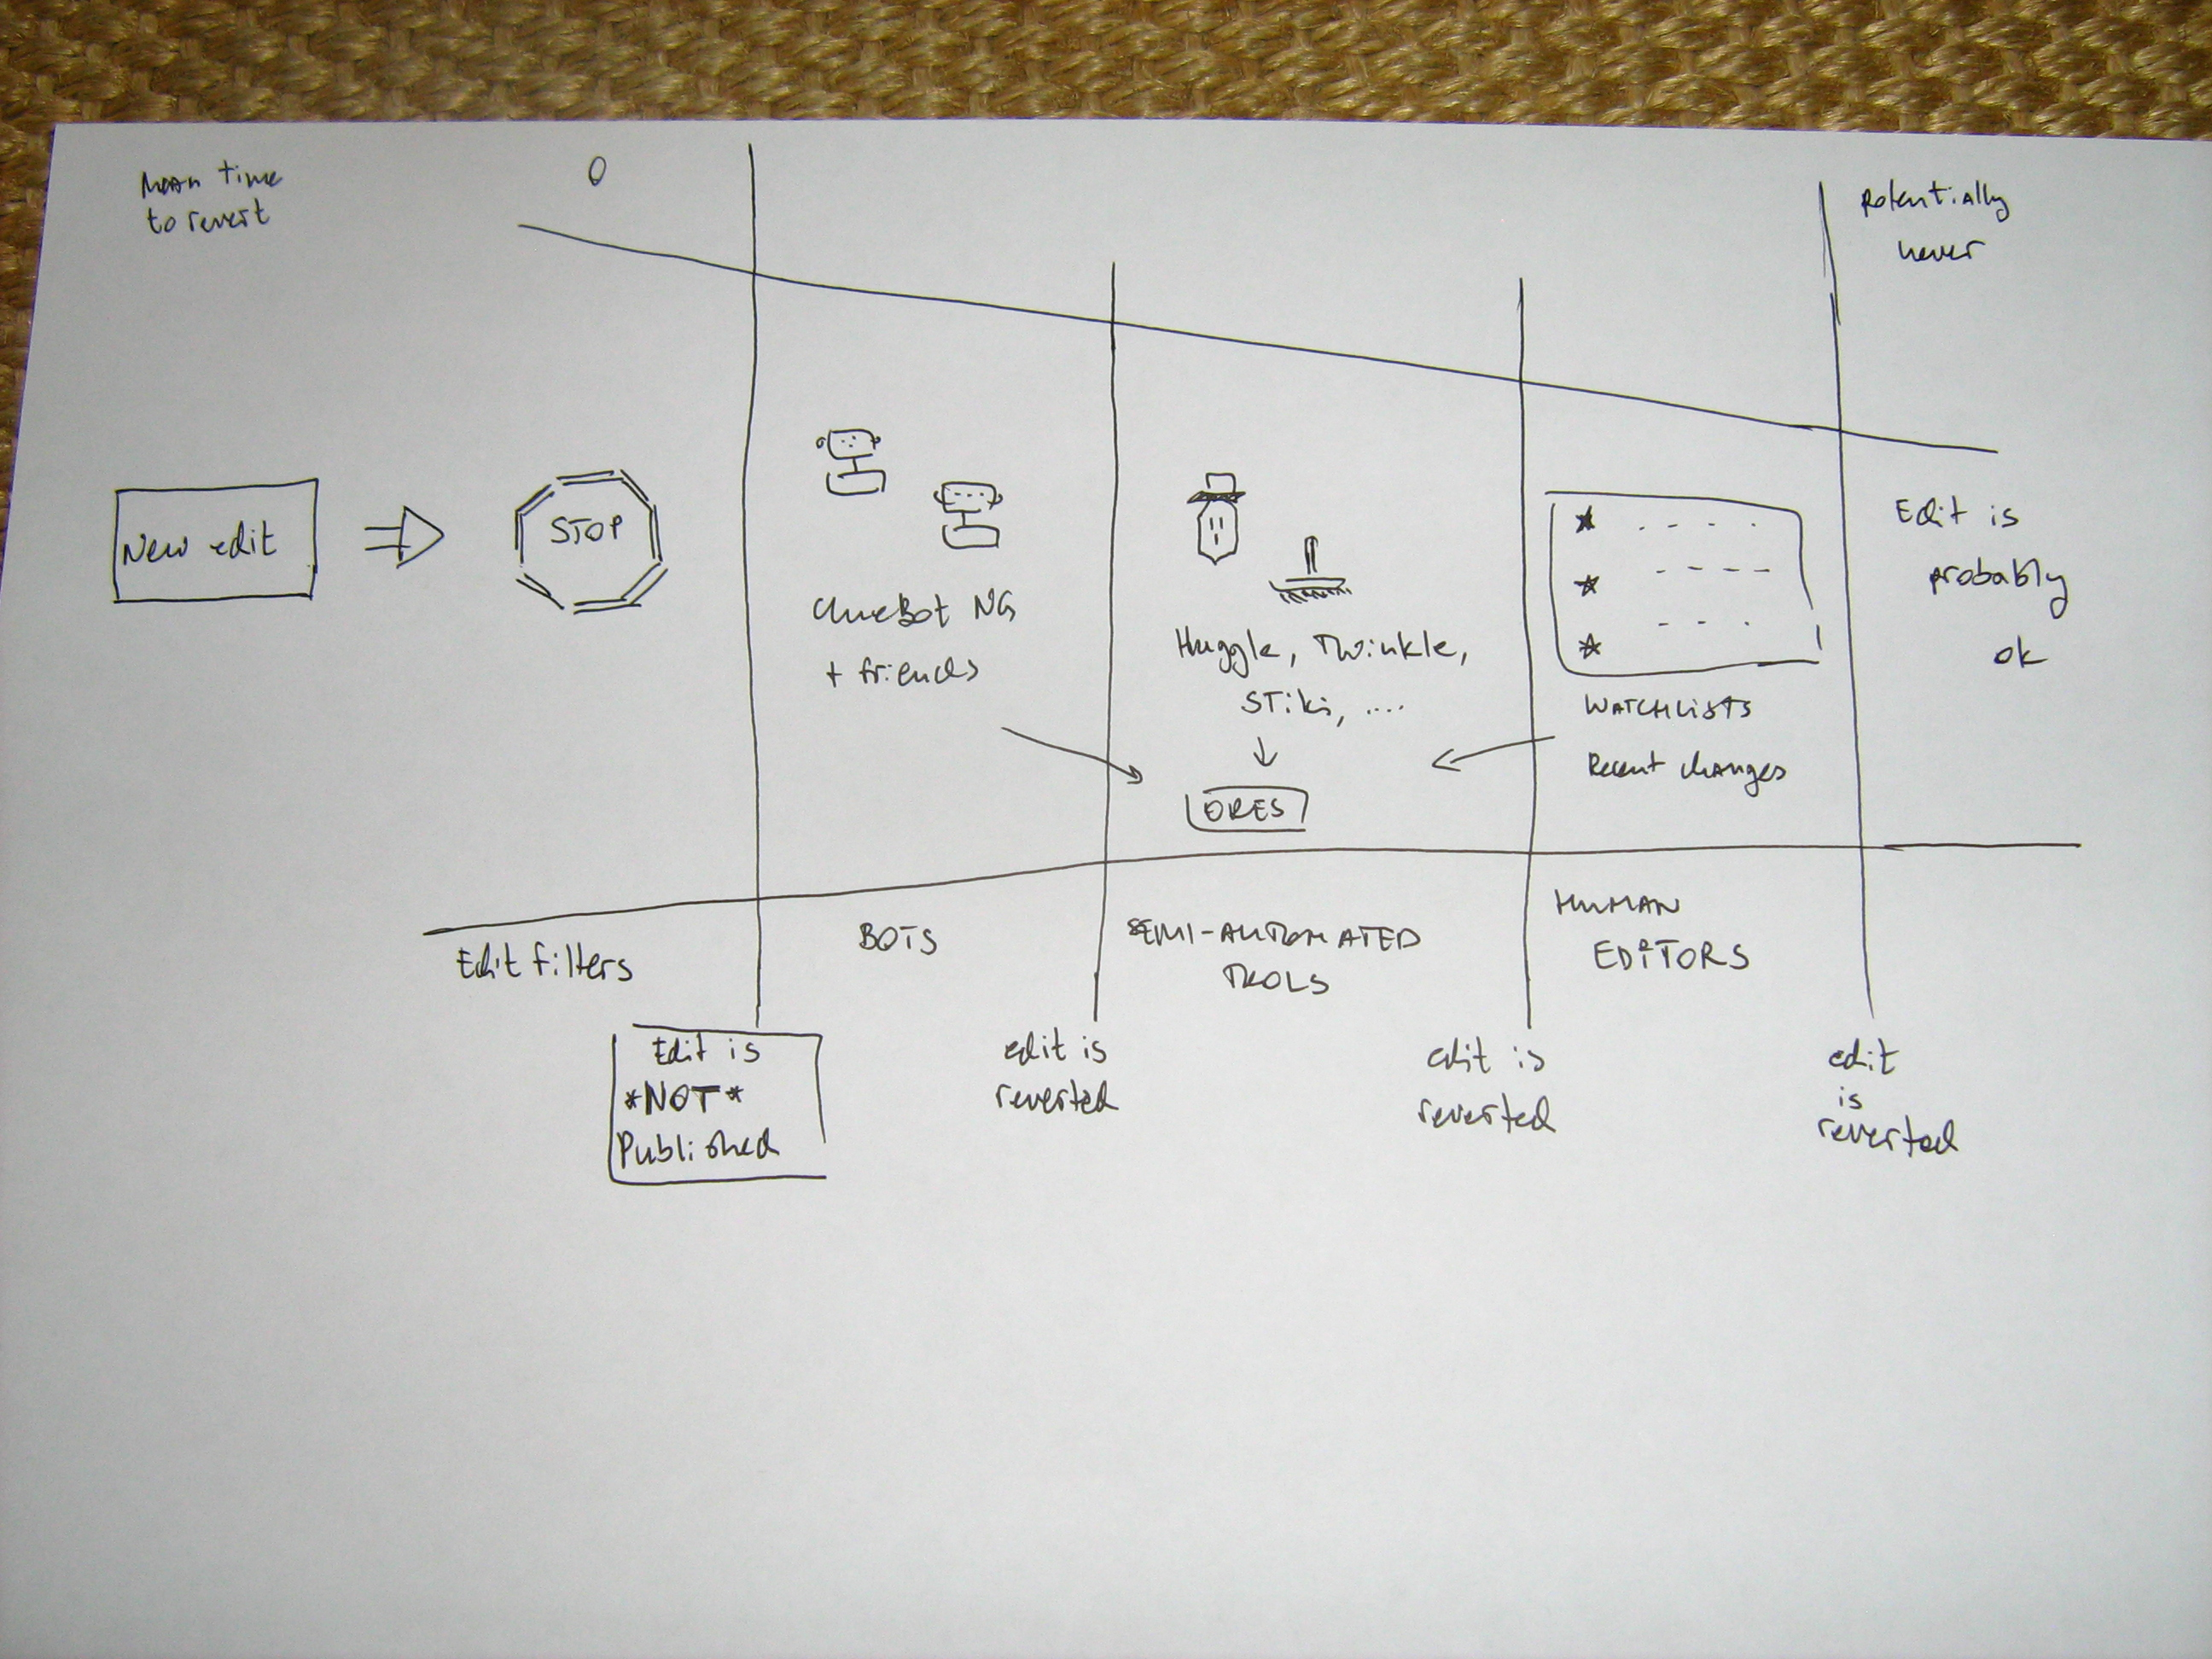
\includegraphics[width=0.9\columnwidth]{pics/funnel-diagramm-with-filters.JPG}
  \caption{Edit filters' role in the quality control frame}~\label{fig:funnel-with-filters}
\end{figure}
%*********************

% Collaboration of the mechanisms
\subsection{Collaboration with bots (and semi-automated tools)}
\label{subsection:collaboration-bots-filters}

So far we have juxtaposed the single quality control mechanisms and compared them separately.
It is however worth mentioning that they not only operate alongside each other but also cooperate on occasions.

Such collaborations are studied for instance by Geiger and Ribes~\cite{GeiRib2010} who go as far as describing them as ``distributed cognition''.
They follow a particular series of abuse throughout Wikipedia, along the traces the disrupting editor and the quality control mechanisms deployed against their edits left.
The researchers demonstrate how a bot (ClueBot), and several editors using the semi-automated tools Huggle and Twinkle all collaborate up until the malicious editor was banned by an administrator.

During the present study, I have also observed various cases of edit filters and bots mutually facilitating each other's work.
%TODO check whether there are other types of cooperations at all: what's the deal with Twinkle? and update here!
% are there further examples of such collaborations: consider scripting smth that parses the bots descriptions from https://en.wikipedia.org/wiki/Category:All_Wikipedia_bots and looks for "abuse" and "filter" -- nice idea, but no time
DatBot, Mr.Z-bot and MusikBot are all examples for bots conducting support tasks for filters.
DatBot~\cite{Wikipedia:DatBot} monitors the Abuse Log\footnote{\url{https://en.wikipedia.org/wiki/Special:AbuseLog}}
and reports users tripping certain filters to WP:AIV (Administrator intervention against vandalism)\footnote{\url{https://en.wikipedia.org/wiki/Wikipedia:Administrator_intervention_against_vandalism}} and WP:UAA (usernames for administrator attention)\footnote{\url{https://en.wikipedia.org/wiki/Wikipedia:Usernames_for_administrator_attention}}.
It is the successor of Mr.Z-bot\footnote{\url{https://en.wikipedia.org/w/index.php?title=User:Mr.Z-bot&oldid=898492130}}
which used to report users from the abuse log to WP:AIV, but has been inactive since 2016 and therefore recently deactivated.
%\url{https://en.wikipedia.org/wiki/Wikipedia:Bots/Requests_for_approval/Mr.Z-bot_7}

MusikBot also has several tasks dedicated to monitoring different aspects of edit filter behaviour and compiling reports for anyone interested:
The FilterMonitor task ``[r]eports functional changes of edit filters to the watchable page User:MusikBot/FilterMonitor/Recent changes. The template \verb|{{recent filter changes}}| formats this information and can be transcluded where desired''\footnote{\url{https://en.wikipedia.org/w/index.php?title=User:MusikBot/FilterMonitor&oldid=748920629}}.
The StaleFilter task ``[r]eports enabled filters that have not had any hits in over 30 days, as specified by \verb|/Offset|''\footnote{\url{https://en.wikipedia.org/w/index.php?title=User:MusikBot/StaleFilters&oldid=763698371}}.
The AbuseFilterIRC task ``[r]elays all edit filter hits to IRC channels and allows you to subscribe to notifications when specific filters are tripped. See \verb|#wikipedia-en-abuse-log-all| for the English Wikipedia feed''\footnote{\url{https://en.wikipedia.org/w/index.php?title=User:MusikBot/AbuseFilterIRC&oldid=885138803}}.

On the other hand, there are also examples for filters supporting bot work:
Filter 323 (``Undoing anti-vandalism bot'') tags edits reverting revisions by XLinkBot and ClueBot NG.
Although it is hidden, so we cannot view any details, filter 603 is named ``Special case of reverting XLinkBot reverts'' so it is probably safe to assume that is filtering what it claims to be.
And there are several filters (historically) configured to ignore particular bots: filter 76 (``Adding email address'') exempting XLinkBot, filter 28 (``New user redirecting an existing substantial page or changing a redirect'') exempting Anybot, filter 532 (``Interwiki Addition'') exempting Cydebot are some examples thereof.
There are also filters configured to ignore all bots: filter 368 (``Making large changes when marking the edit as minor''), filter 702 (``Warning against clipboard hijacking''), filter 122(``Changing Username malformed requests'').

\begin{comment}
Apparently, Twinkle at least has the possibility of using heuristics from the abuse filter log for its queues.
%TODO is that so? the only place I can find abuse filters mentioned with Twinkle is in the source code: https://github.com/azatoth/twinkle/blob/master/morebits.js#L2636; and I'm not quite sure what this part of the code does.
\end{comment}


%************************************************************************

\section{Fazit}
%Conclusion, resume, bottom line

In short, in this chapter we found/worked out following salient characteristics of edit filters: ....

